% This is "sig-alternate.tex" V2.1 April 2013
% This file should be compiled with V2.5 of "sig-alternate.cls" May 2012
%
% This example file demonstrates the use of the 'sig-alternate.cls'
% V2.5 LaTeX2e document class file. It is for those submitting
% articles to ACM Conference Proceedings WHO DO NOT WISH TO
% STRICTLY ADHERE TO THE SIGS (PUBS-BOARD-ENDORSED) STYLE.
% The 'sig-alternate.cls' file will produce a similar-looking,
% albeit, 'tighter' paper resulting in, invariably, fewer pages.
%
% ----------------------------------------------------------------------------------------------------------------
% This .tex file (and associated .cls V2.5) produces:
%       1) The Permission Statement
%       2) The Conference (location) Info information
%       3) The Copyright Line with ACM data
%       4) NO page numbers
%
% as against the acm_proc_article-sp.cls file which
% DOES NOT produce 1) thru' 3) above.
%
% Using 'sig-alternate.cls' you have control, however, from within
% the source .tex file, over both the CopyrightYear
% (defaulted to 200X) and the ACM Copyright Data
% (defaulted to X-XXXXX-XX-X/XX/XX).
% e.g.
% \CopyrightYear{2007} will cause 2007 to appear in the copyright line.
% \crdata{0-12345-67-8/90/12} will cause 0-12345-67-8/90/12 to appear in the copyright line.
%
% ---------------------------------------------------------------------------------------------------------------
% This .tex source is an example which *does* use
% the .bib file (from which the .bbl file % is produced).
% REMEMBER HOWEVER: After having produced the .bbl file,
% and prior to final submission, you *NEED* to 'insert'
% your .bbl file into your source .tex file so as to provide
% ONE 'self-contained' source file.
%
% ================= IF YOU HAVE QUESTIONS =======================
% Questions regarding the SIGS styles, SIGS policies and
% procedures, Conferences etc. should be sent to
% Adrienne Griscti (griscti@acm.org)
%
% Technical questions _only_ to
% Gerald Murray (murray@hq.acm.org)
% ===============================================================
%
% For tracking purposes - this is V2.0 - May 2012

\documentclass{sig-alternate-05-2015}


\begin{document}

% Copyright
%\setcopyright{acmcopyright}
%\setcopyright{acmlicensed}
%\setcopyright{rightsretained}
%\setcopyright{usgov}
%\setcopyright{usgovmixed}
%\setcopyright{cagov}
%\setcopyright{cagovmixed}


% DOI
%\doi{10.475/123_4}

% ISBN
%\isbn{123-4567-24-567/08/06}

%Conference
%\conferenceinfo{PLDI '13}{June 16--19, 2013, Seattle, WA, USA}

%\acmPrice{\$15.00}

%
% --- Author Metadata here ---
%\conferenceinfo{WOODSTOCK}{'97 El Paso, Texas USA}
%\CopyrightYear{2007} % Allows default copyright year (20XX) to be over-ridden - IF NEED BE.
%\crdata{0-12345-67-8/90/01}  % Allows default copyright data (0-89791-88-6/97/05) to be over-ridden - IF NEED BE.
% --- End of Author Metadata ---

\title{Clustering Documents in Topic Space: Worth the Effort?}
\subtitle{A Fair Comparison with Established Vector-Space Model Techniques}
%\titlenote{A full version of this paper is available}

\numberofauthors{3} 

\author{
\alignauthor
Matthew Hawthorn\\
       \email{mah6wt@virginia.edu}
\alignauthor
Shannon Mitchell\\
       \email{som3dq@virginia.edu}
\alignauthor 
Nikhil Mascarenas\\
       \email{nm4gt@virginia.edu}
}

\date{26 Feb 2016}

\maketitle

\keywords{document clustering; vector space models; topic models}


\section{Background and Motivation}
Document clustering is an important method used widely in information retrieval. It is also important in other fields where document labels are not available such as identifying new trends within research studies, forensic computing and innovations within patent applications. Hierarchical clustering methods can typically obtain better performance than simpler methods such as k-means, however hierarchical methods can be prohibitively expensive on large datasets in terms of computational speed. Documents are often represented with a vector space model using a term frequency-inverse document frequency (tf-idf) embedding, but the more recent approach of latent topic modelling, best exemplified by Latent Dirichlet Allocation (LDA)\cite{LDA}, can potentially embed documents in a much lower-dimensional space of latent `topics', groupings of frequently co-occurring terms.  This speeds up document similarity computations, resulting for instance in faster queries in document retrieval, or faster clustering once the model is computed.  We suspect topic models can improve accuracy of similarity measures as well; especially when documents are short, two highly semantically similar documents might nonetheless share few terms (yielding a low cosine similarity), whereas they are more likely to overlap in topics (in the topic model sense).  In this way we hypothesize that for many corpora, clustering on topic weights might yield better results than clustering on term frequencies.


\section{Previous Work}
To our knowledge, relatively little work has been done on evaluating the utility of topic models for document clustering; the vast majority of studies of document clustering have investigated it in the context of vector-space models.

\par
In a comprehensive and authoritative survey, Zhao and Karypis (2002)\cite{clustersurvey} compare 9 different agglomerative and 6 partitional hierarchical clustering techniques using 12 text datasets including the Reuters-21578 news corpus, representing documents in a traditional vector space model using tf-idf embedding. As partitional clustering algorithms such as k-means are often selected due to lower computational requirements, they wanted to confirm whether there was a tradeoff with model performance. The results surprisingly showed that more expensive agglomerative clustering algorithms were outperformed by a hierarchical divisive bisecting k-means algorithm, measuring by cluster agreement with labelled classes using an F-score criterion averaged over all levels of the resulting tree.

\par
Xie and Xing (2013)\cite{jointinference} propose a new document clustering method integrating topic modelling and clustering into a single probabilistic graphical model with topics and clusters as latent variables. They jointly infer topics and clusters using this model, and then compare the accuracy of the resulting clusters against several other clustering algorithms. Among these other techniques are traditional k-means in normalized tf-idf space, k-means performed on LDA topic weight vectors, and ``LDA+naive'' which denotes the treatment of topics as clusters and assigning documents to their highest-weight topics.  They find that their joint probabilistic model, the ``Multi-grain Clustering Topic Model'' (MGCTM), outperforms the other methods they tried, measuring by normalized mutual information (NMI) on the 20-Newsgroups and Reuters-21578 datasets, though only by a slight margin over the ``LDA+naive'' approach.

In contrast to the more complex joint inference approach of Xie and Xing, Ma et. al. (2014)\cite{threestage} investigate the use of traditional clustering techniques on embeddings of documents in a standard LDA topic space.  They employ a three-stage process: 1) identify an optimal number of topics according to a ``topic significance degree'' measure, 2) seed initial cluster centers using the k-means++ algorithm, 3) carry out k-means clustering in the usual manner, but using Jensen-Shannon divergence as a distance measure rather than euclidean distance.  Compared against the same procedure without tuning the number of topics, they find some improvement on their two datasets, which include 20-Newsgroups.

\section{Research Problem}
The added utility of topic models over simpler vector-space models for document classification and clustering in the general case is still largely open to question; papers we have found discussing one technique or the other use either different datasets or different evaluation metrics and are therefore not directly comparable.  Xie and Xing make a direct comparison between their complex model and simpler approaches, but implement the simpler approaches naively, not giving a fair comparison.  This was exacerbated by the fact that accuracy margins for their model over the simplest LDA approach were narrow (50.1\% vs. 48.0\% NMI and 56.6\% vs. 54.9\% accuracy on Reuters-21758).  We propose to make a fuller comparison.  What we want to know is: can we do much better clustering documents in topic space than we can by using the state of the art techniques in traditional tf-idf vector space? Is the computational cost worth it?


\section{Techniques}
We will explore document clustering techniques applied to topic embeddings, and compare them with clusterings using tf-idf embeddings.  With large data sets in mind, we rule out agglomerative techniques as too computationally expensive, and we would like to use techniques which have already been efficiently implemented for large data.  For instance, Apache Mahout already has good implementations of Latent Dirichlet Allocation and k-means, whereas the complex joint inference task of Xie and Xing would require a good deal of development to be deployed at scale, and may or may not prove to be scaleable. This leaves us with partitional techniques on LDA topic embeddings. Specifically we will try the bisectional k-means found by Zhao and Karypis to be optimal for tf-idf vectors.  The hierarchical partitional technique gives us an opportunity to optimize the cluster count via cluster coherence measures as well, rather than artificially evaluating on the known number of categories.

The choice of metric is important in clustering, especially in high-dimensional spaces.  Euclidean distance, for instance (which Xie \& Xing use in k-means on LDA topic space for comparison) is an inappropriate metric on the simplex where topic distributions reside.  Lebanon (2006)\cite{learnedmetrics} found that learning an optimal metric on the simplex from term distributions resulted in nearly half the error rate of tf-idf cosine in a binary text classification task.  We believe that for probability distributions, information-theoretic distance metrics have better theoretical support than usual metrics such as L2 norm (euclidean distance) or L1 norm.  Thus, in agreement with Ma et. al., we will implement k-means using the Jensen-Shannon divergence (JS).  We believe this is well-founded since the JS divergence is the square of a metric, and just as with squared euclidean distance, the sum of JS divergences from a centroid is minimized at the mean distribution, as demonstrated by Fuglede \& Topsoe (2004)\cite{hilbertspace}. A comparison of our proposal to previous work is summarized in Appendix \ref{comparison}.


\section{Evaluation}
We will compare our clusterings of documents in topic space against the best hierarchical algorithm from Zhao and Karypis in tf-idf space on the following datasets:
\begin{itemize}
\item 20-Newsgroups
\item Reuters-21578
\end{itemize}
We will evaluate our clusterings using the following metrics:
\begin{itemize}
\item F-score as implemented by Zhao and Karypis for hierarchical clusterings
\item F-score as implemented by Ma et. al. for flat (k-means) clusterings.  
\item Normalized mutual information, which Xie and Xing use to evaluate their clusterings.
\end{itemize}

\par
In this way, we will achieve a fair comparison of different document clustering techniques while bringing to bear the best available techniques in both the vector space and topic model representations. We will also get a fair comparison with the more complex joint inference technique of Xie and Xing.


\section{Expected Outcome}
We expect to find a clear winner, and to finally be able to answer the question of which document embedding can be expected to perform best for clustering tasks on datasets which are comparable to our test sets.  If it is the vector-space model, then there seems little utility in the topic model computation for the purposes of clustering. If it is the topic model representation, then it becomes a relevant question in an application context whether the computational cost is worth the improved accuracy.  If our technique beats or matches the more complex and potentially less scalable joint inference technique of Xie and Xing, then there seems little utility in developing that technique for larger scale applications.


% The following two commands are all you need in the
% initial runs of your .tex file to
% produce the bibliography for the citations in your paper.

\bibliographystyle{abbrv}
\bibliography{proposal}

% You must have a proper ".bib" file
%  and remember to run:
% latex bibtex latex latex
% to resolve all references
% ACM needs 'a single self-contained file'!

%APPENDICES are optional
\balancecolumns

\appendix
%Appendix A
\section{Comparison With Prior Work}\label{comparison}

\begin{figure}[h]
\centering
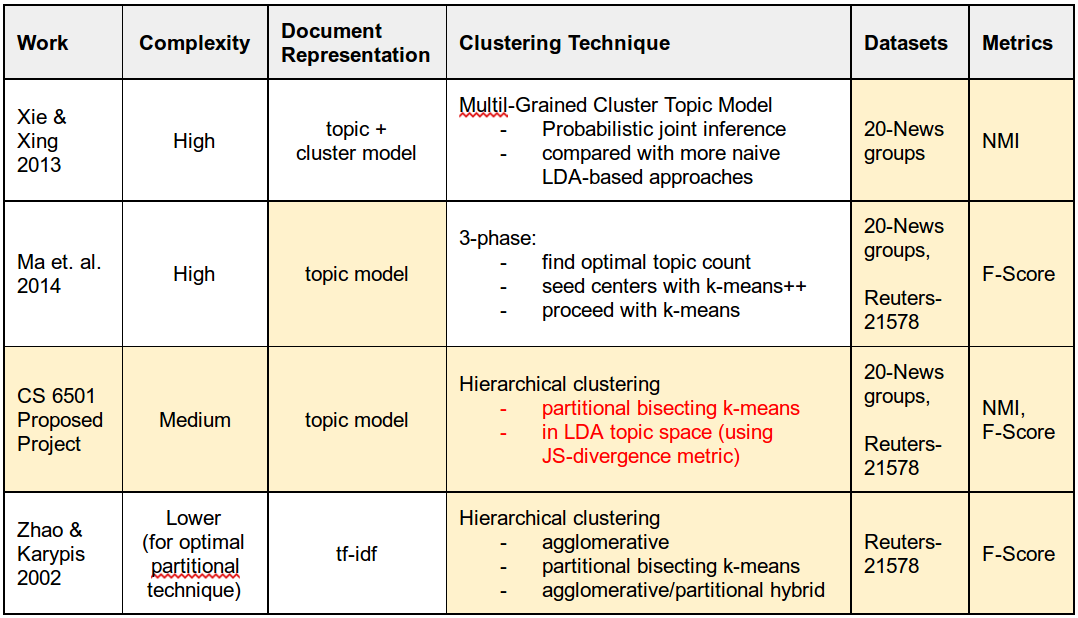
\includegraphics[width=6in]{comparisontable}
\caption{A comparison of our proposed project with prior research. Overlaps in document representation, clustering technique, datasets, and evaluation metrics are highlighted. Some information is omitted for clarity.}
\vskip -6pt
\end{figure}

\end{document}
